\section{Model Dependent Upper Limits}
\label{sec:sigmalimit}

As an example of how the upper limit presented in Sec.~\ref{sec:limits} can be
used to test if a specific model is excluded, in this section we consider the benchmark
SUSY processes LM1, LM3 and LM6.
We place upper limits on the quantity $\sigma \times A$,
assuming efficiencies and uncertainties from these processes, and compare them to 
the expected values of $\sigma \times A$.
Here $\sigma$ is the signal production cross section and $A$ is the signal acceptance.

The signal event yield $N_{SIG}$ can be expressed as:

\begin{equation}
N_{SIG} = \sigma \times A \times \epsilon \times \mathcal{L},
\end{equation}

and we therefore have:

\begin{equation}
N_{SIG}/( \epsilon \times \mathcal{L}) = \sigma \times A.
\end{equation}

Here  $\epsilon$ is the signal efficiency and $\mathcal{L}$ is the integrated luminosity. 
Since we wish to place an upper limit on the quantity $\sigma \times A$, we must evaluate
the quantity $N_{SIG}/(\epsilon \times \mathcal{L})$.  Because of the efficiency
in the denominator, this upper limit cannot be calculated in an entirely model-independent
way; rather, it must be calculated with respect to a specific model. We therefore evaluate
the upper limit on $\sigma \times A$ with respect to LM1, LM3 and LM6.  
For each process, we must calculate both the efficiency and its uncertainty.

We evaluate the signal efficiencies and acceptances using MC. The acceptance is defined by he
following requirements which are applied on the generator-level quantities:

\begin{itemize}
\item 2 electrons or muons with \pt\ $>$ 10 GeV and $|\eta|<2.5$, at least 1 lepton must have \pt\ $>$ 20 GeV
\item Opposite-sign pair, veto same-flavor pairs with $76 < \rm{m(\ell\ell)} < 106$~GeV
\item Count genjets with $p_T > 30$~GeV, $|\eta|<3.0$, $\Delta R > 0.4$ from any selected lepton as defined above, require at least 2 genjets
\item $H_{T}^{gen}$ is the scalar sum of selected genjet \pt's, $MET^{gen}$ is the event gen-level missing ET, and $y^{GEN} \equiv MET^{gen}/\sqrt{H_{T}^{gen}}$.
\end{itemize}

For the 2010, high \met, and high \Ht\ signal regions, we add the corresponding
requirements on the generator-level quantities $H_{T}^{gen}$, $MET^{gen}$ and $y^{GEN}$.
The signal efficiency is defined as the fraction of events passing the above acceptance requirements, which
also pass the full reco-level selection. The efficiency uncertainty is determined by the trigger uncertainty (2\%),
the lepton selection uncertainty (2\%/lepton) and the hadronic energy scale uncertainties quoted in Table~\ref{tab:jetmet}.

Armed with the efficiencies and uncertainties calculated in the previous 2 sections, we proceed
to calculate upper limits on the quantity $\sigma \times A$ for the 3 benchmark SUSY 
scenarios. We calculate Bayesian 95\% CL upper
limits using the cl95cms software, assuming a log-normal model of nuissance parameter integration.
We quote here the upper limits from the high \Ht\ signal region.
The results are summarized in
Table~\ref{tab:models}. These results show that the LM1, LM3 and LM6 scenarios are excluded.

\begin{table}[hbt]
\begin{center}
\caption{\label{tab:models} Summary of model-dependent limits. The efficiency and acceptance are
defined in the text; the efficiency uncertainty is dominated by the uncertainty in the hadronic
energy scale. The 95\% CL Bayesian UL on the quantity $\sigma\times A$ is indicated, as well as
the value of this quantity for the LM1, LM3 and LM6 scenarios.}
\begin{tabular}{l|ccc}
\hline
                                         & LM1              & LM3             & LM6               \\
\hline
\hline
{\bf 2010 signal region}                 &                  &                 &                   \\
\hline
efficiency (\%)                          &  50 $\pm$ 5      & 46 $\pm$ 5      & 52 $\pm$ 4        \\
acceptance (\%)                          &  2.0             & 1.2             & 3.5               \\
UL($\sigma \times A$) (fb)               &  47              & 51              & 44                \\
$\sigma \times A$ (fb)                   &  140             & 60              & 16                \\
\hline
\hline
{\bf high \met\ signal region}           &                  &                 &                   \\
\hline
efficiency (\%)                          &  46 $\pm$ 10     & 43 $\pm$ 12     & 54 $\pm$ 6        \\
acceptance (\%)                          &  1.3             & 0.67            & 2.8               \\
UL($\sigma \times A$) (fb)               &  26              & 29              & 21                \\
$\sigma \times A$ (fb)                   &  87              & 35              & 13                \\
\hline
\hline
{\bf high \Ht\ signal region}            &                  &                 &                   \\
\hline
efficiency (\%)                          &  42 $\pm$ 13     & 40 $\pm$ 13     & 52 $\pm$ 7        \\
acceptance (\%)                          &  0.94            & 0.67            & 2.5               \\
UL($\sigma \times A$) (fb)               &  16              & 18              & 12                \\
$\sigma \times A$ (fb)                   &  68              & 36              & 12                \\
\hline
\end{tabular}
\end{center}
\end{table}


We also quote the result more generally in the context of the CMSSM.
The Bayesian 95\% CL limit  in the  $(m_0,m_{1/2})$ plane,  for $\tan\beta=10$,
$A_0 = 0$ and $\mu > 0$ is shown in Figure~\ref{fig:msugra}. 
The high \met\ and high \Ht signal regions have similar sensitivity to the CMSSM; 
here we choose to show results based on the high-\Ht signal regions. The
SUSY particle  spectrum is calculated using  SoftSUSY~\cite{Allanach:2002uq}, and the
signal  events  are  generated  at  leading  order  (LO)  with  PYTHIA6.4.22.
NLO  cross sections,  obtained  with the
program  Prospino~\cite{Beenakker:1997kx},  are used  to  calculate  the observed
exclusion  contour.  
At each point in the  $(m_0,m_{1/2})$ plane, the acceptance uncertainty is calculated by
summing in quadrature the uncertainties from jet and \met\ energy scale using the
procedure discussed in Section~\ref{sec:systematics}, the uncertainty in the 
NLO cross section due to the choice of factorization and renormalization scale, 
and the uncertainty from the parton distribution function (PDF) for CTEQ6.6~\cite{Nadolsky:2008fk},
estimated from  the  envelope  provided  by  the  CTEQ6.6  error sets.
The luminosity uncertainty and dilepton
selection efficiency uncertainty are also included, giving a total relative acceptance uncertainty which varies
in the range 0.2--0.3.
A point is considered to be excluded if the NLO yield exceeds the 95\% CL
Bayesian upper limit calculated with this acceptance uncertainty, using
a log-normal model for the nuisance parameter integration.

\begin{figure}[tbh]
\begin{center}
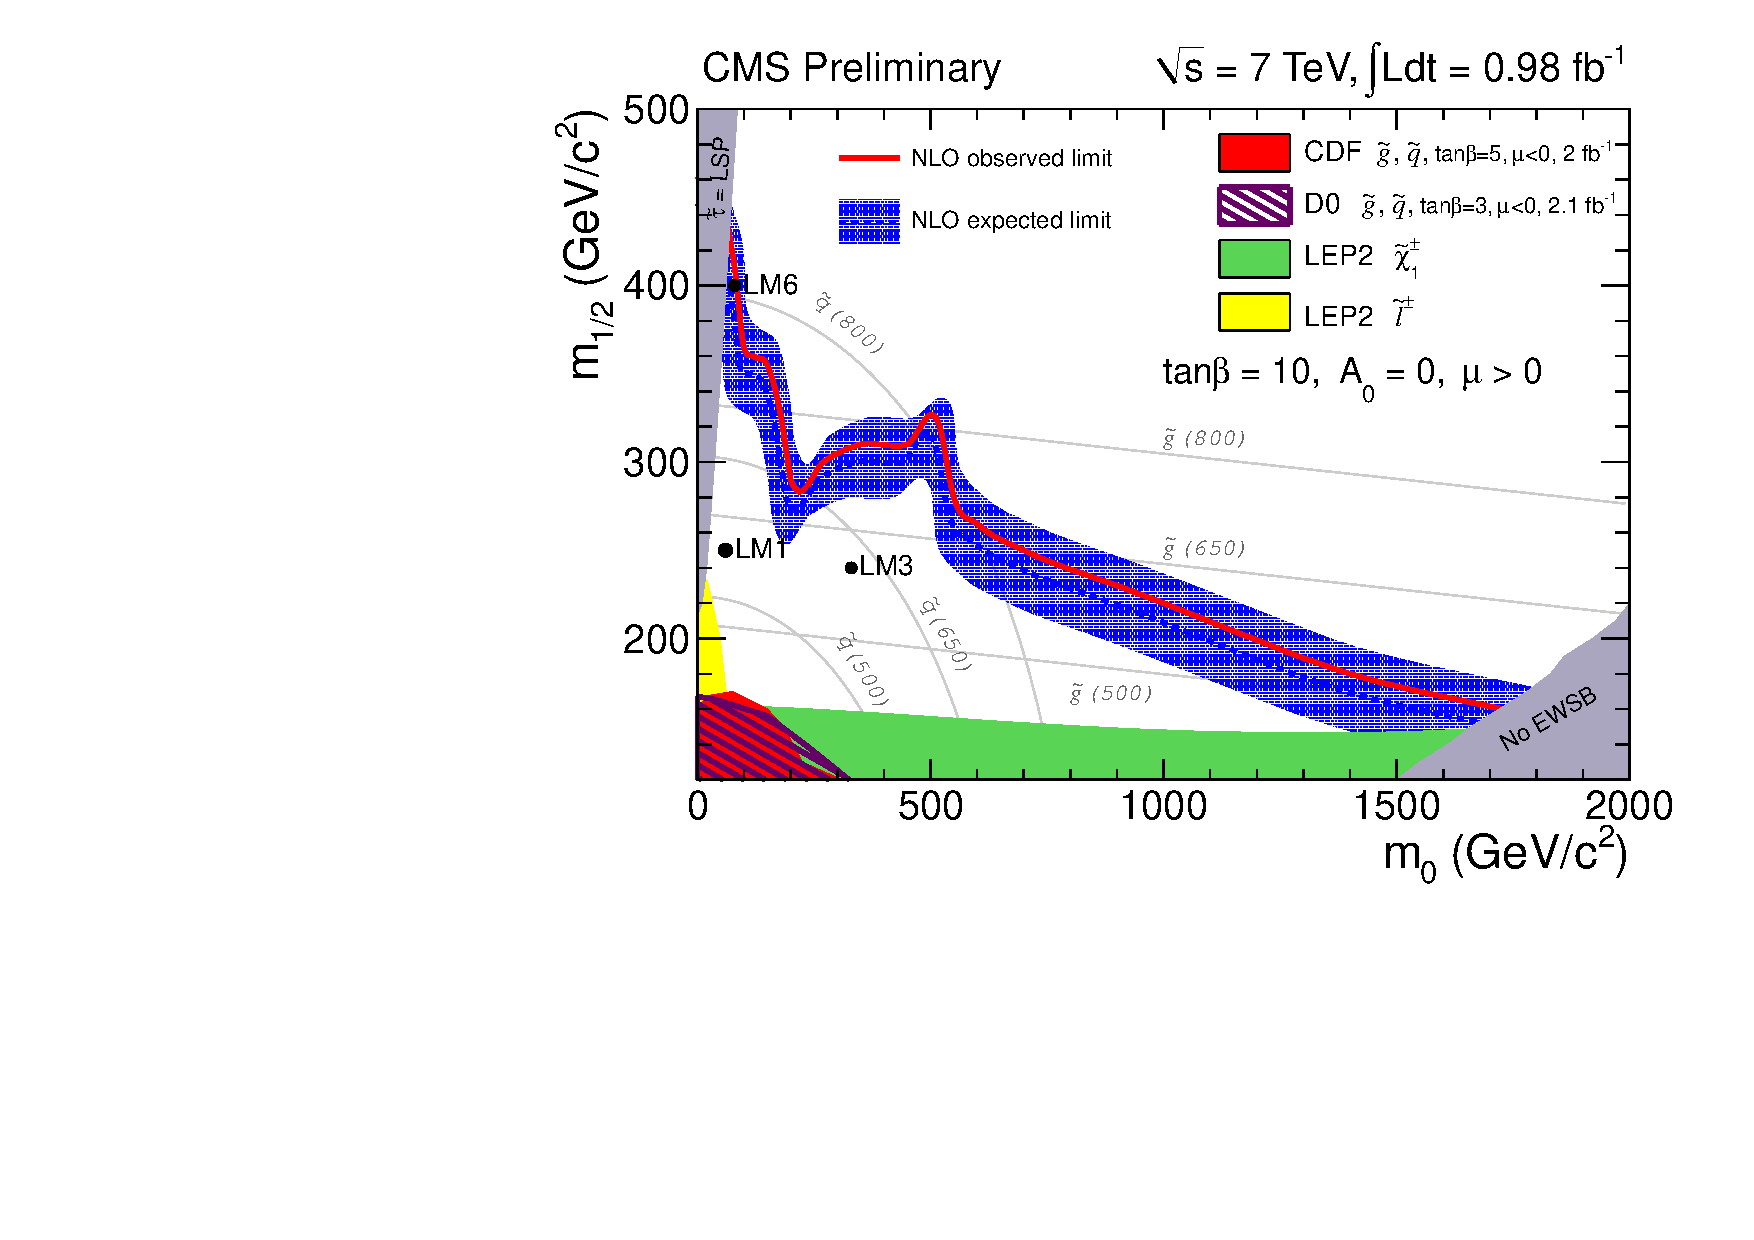
\includegraphics[width=1\linewidth]{plots/RA6_ExclusionLimit_tanb10.pdf}
\caption{\label{fig:msugra}\protect 
%Text taken from RA1 paper
The observed 95\% CL exclusion contour at NLO (solid red line) and the expected exclusion contour (dashed blue line) 
in the CMSSM $(m_0,m_{1/2})$ plane for  $\tan\beta=10$, $A_0 = 0$ and $\mu > 0$. 
The area below the curve is excluded by this measurement. Exclusion limits obtained from 
previous experiments are presented as filled areas in the plot. Thin grey lines correspond to 
constant squark and gluino masses.}
\end{center}
\end{figure}

The excluded regions  for the CDF
search for  jets + missing  energy final states~\cite{PhysRevLett.102.121801} were
obtained for $\tan\beta=5$, while those from D0~\cite{Abazov2008449} were obtained for 
$\tan\beta=3$, each with  approximately  2~fb$^{-1}$ of  data and for $\mu < 0$. 
The  LEP-excluded
regions  are based  on searches  for  sleptons and  charginos~\cite{LEPSUSY}.  
%A comparison of the exclusion limit for tan b = 3 to that for tan b = 10
%for fixed values of A0 =  0 and sign(m) > 0 indicates that
%the exclusion  reach is only weakly  dependent on the value  of tan b;
%the limit shifts  by less than 20\GeV  in m0 and by less  than 10\GeV in
%m1/2.
The D0 exclusion limit, valid for $\tan\beta=3$  and obtained from
a  search  for  associated  production   of  charginos $\chi_{1}^{\pm}$ and
neutralinos $\chi_2^0$ in  trilepton final states~\cite{Abazov200934}, is also
included  in Figure~\ref{fig:msugra}. In  contrast to  the other  limits  presented in
Figure~\ref{fig:msugra},  the results of our search and of the  trilepton search are  strongly dependent on
the choice  of $\tan\beta$ and  they reach the  highest sensitivity  in the
CMSSM for $\tan\beta$ values below 10.




\begin{comment}
-----------------------------------------------

LM1 2010    sigma X acc   0.26
LM1 highmet sigma X acc   0.17
LM1 highht  sigma X acc   0.13

LM3 2010    sigma X acc   0.11
LM3 highmet sigma X acc   0.062
LM3 highht  sigma X acc   0.064

LM6 2010    sigma X acc   0.029
LM6 highmet sigma X acc   0.024
LM6 highht  sigma X acc   0.022


LM1 2010    0.047
LM1 highmet 0.026
LM1 highht  0.016

LM3 2010    0.051
LM3 highmet 0.029
LM3 highht  0.018

LM6 2010    0.044
LM6 highmet 0.021
LM6 highht  0.012


LM1

N(gen)           114514
pre-filter:      219190

N(acc)  2010     4369
N(reco) 2010     2181
acceptance 0.038 efficiency 0.50

N(acc)  high MET 2692
N(reco) high MET 1243
acceptance 0.024 efficiency 0.46

N(acc)  high HT  2108
N(reco) high HT  895
acceptance 0.018 efficiency 0.42

-----------------------------------------------

LM3

N(gen)           123627
pre-filter       220000

N(acc)  2010     2615
N(reco) 2010     1201
acceptance 0.021 efficiency 0.46

N(acc)  high MET 1513
N(reco) high MET 649
acceptance 0.012 efficiency 0.43

N(acc)  high HT  1504
N(reco) high HT  598
acceptance 0.012 efficiency 0.40

-----------------------------------------------

LM6

N(gen)           121523
pre-filter       220000

N(acc)  2010     7622
N(reco) 2010     3959
acceptance 0.063 efficiency 0.52

N(acc)  high MET 6150
N(reco) high MET 3295
acceptance 0.051 efficiency 0.54

N(acc)  high HT  5453
N(reco) high HT  2856
acceptance 0.045 efficiency 0.52

-----------------------------------------------
\end{comment}
